\section{Results}
\subsection{Performance}

Fig. \ref{fig:results} shows the achieved performance for different problem sizes on all three kernels.
NanoVDB achieves overall better results on the CPU compared to OpenVDB.
Above one million rays the GPU starts to overtake both CPU kernels.

OpenVDB achieves up to 18.5 MRps \footnote{1 MRps = $10^6$ Rays per second}. NanoVDB consistently outperforms OpenVDB and reaches up to 29.7 MRps.
For problems with 1 million rays or more the GPU kernel overtakes both CPU implementations and achieves up to 117.4 MRps.
Therefore the switch from OpenVDB to NanoVDB increased performance by a factor of 6.3.

Furthermore both CPU implementations suffer from random drops in performance while GPU results are more consistent.


\begin{figure}[h]
    \begin{subfigure}{0.5\textwidth}
        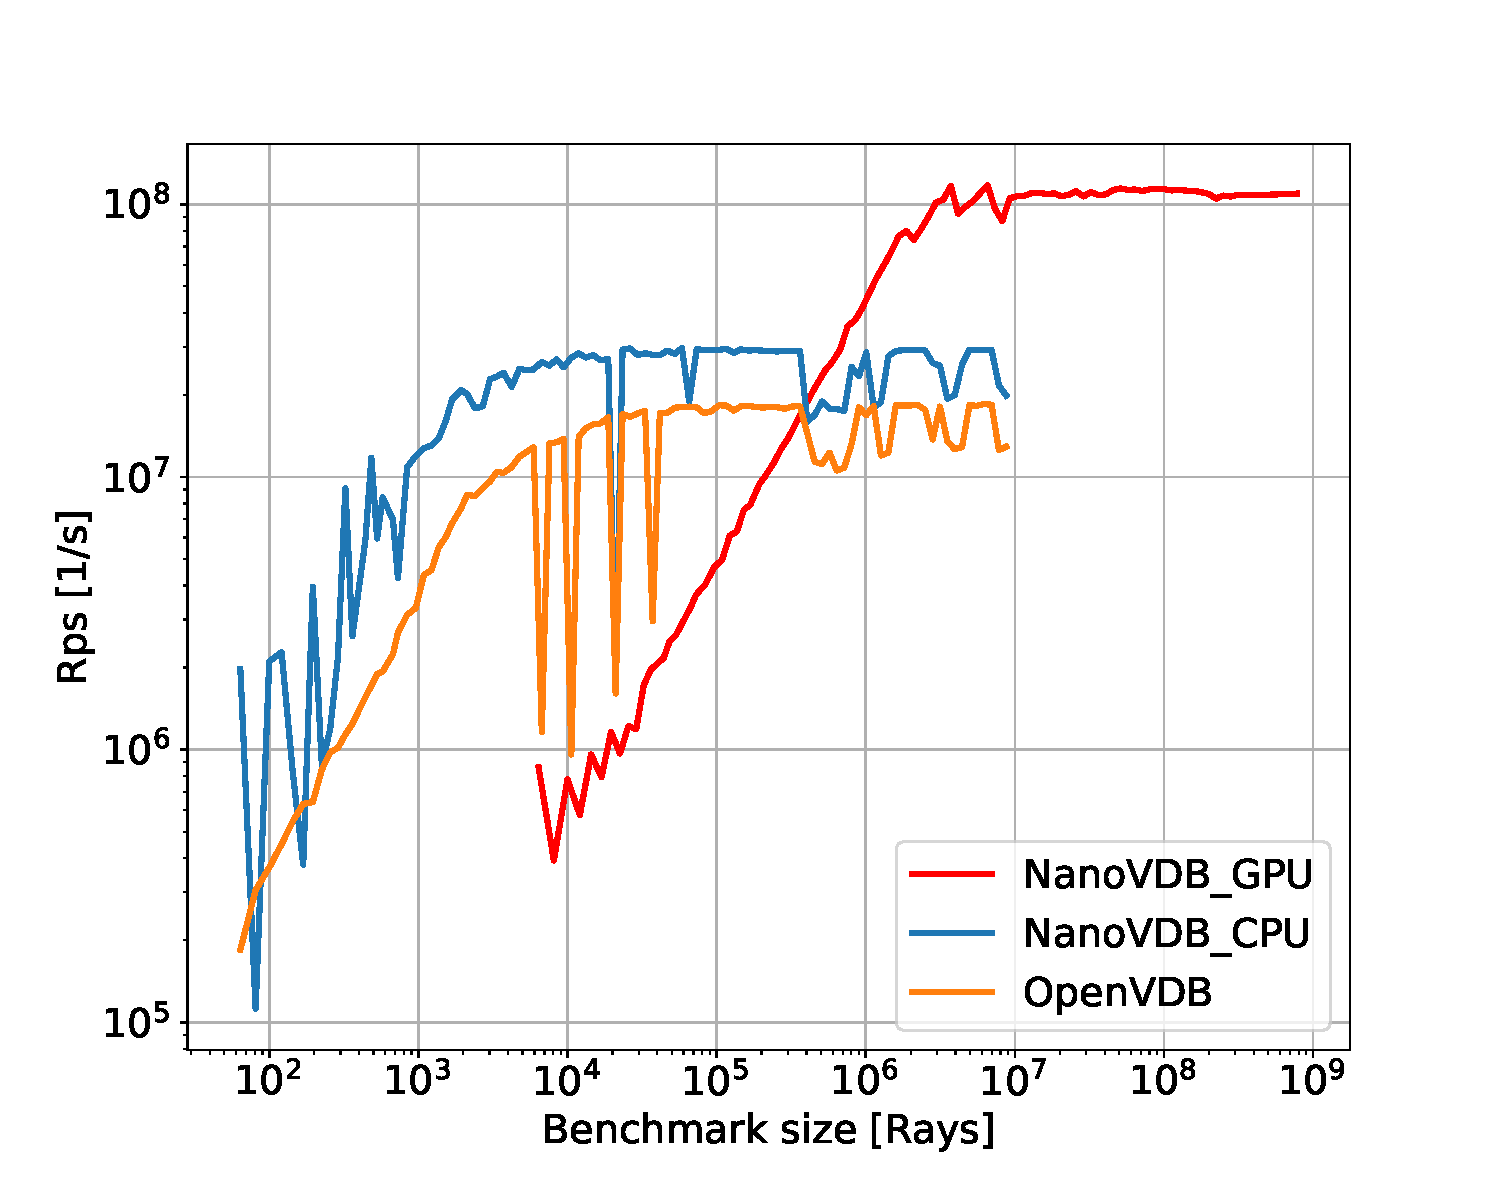
\includegraphics[width=1\linewidth]{res/results.pdf}
        %\label{fig:serial-solution}

    \end{subfigure}
    \begin{subfigure}{0.4\textwidth}
        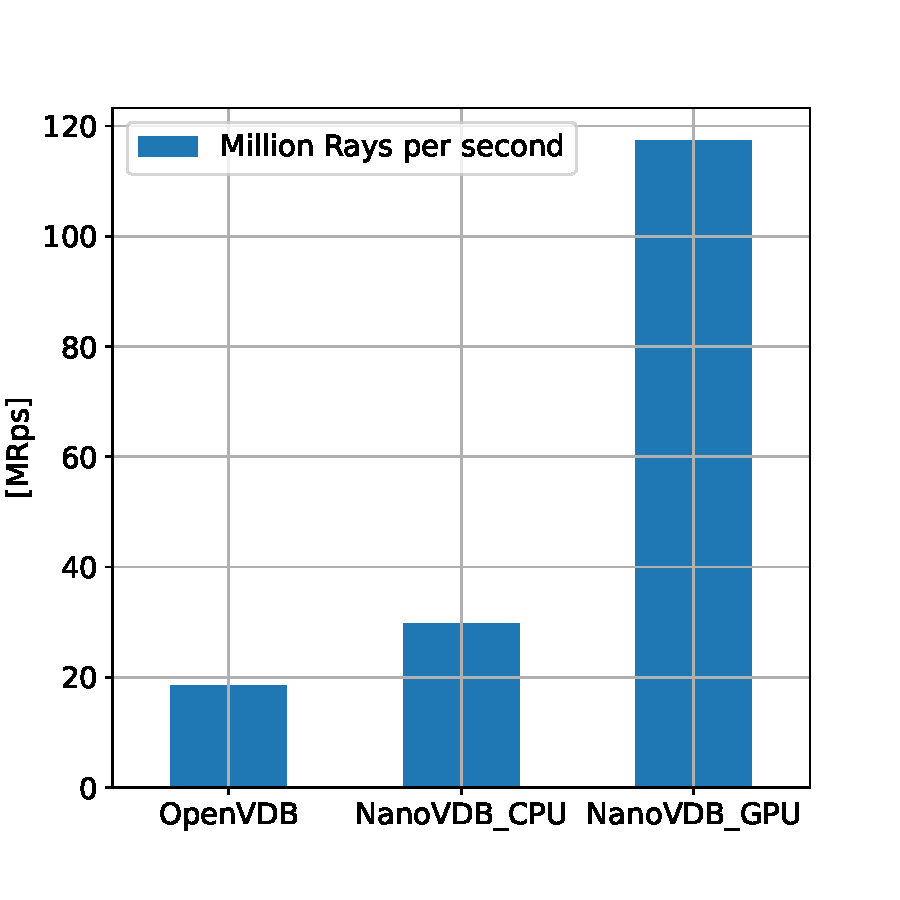
\includegraphics[width=1\linewidth]{res/barplot.pdf}
        %\label{fig:parallel-solution}
    \end{subfigure}

    \caption{\textbf{left:} measured performance across different problem sizes. \textbf{right:} Best results for each kernel}
    \label{fig:results}
\end{figure}

\newpage
\subsection{Accuracy}

NanoVDB's level-set raytracing function (\texttt{nanovdb::ZeroCrossing()}) provides 3 output parameters:

\begin{itemize}
    \item Coordinates (int[3]): index-space coordinates of the voxel that contains the intersection point. 
    In Fig. \ref{fig:results_accuracy} the coordinates have been transformed into world space coordinates
    \item time (float): euclidean distance between ray source and intersection point
    \item value (ValueT): grid value of the voxel i.e. the minimum distance to the surface of the sphere. 
    The datatype of ValueT is determined by the grid. For this experiment a float-grid is used.
\end{itemize}

Fig. \ref{fig:results_accuracy} shows the results for all 3 output parameters for a sphere of radius $r=50$ with it's center at $\mathbf{c} = (100,0,0)^T$.
1000 evenly spaced rays are placed at $\mathbf{eye}_i = (0, y_i, 0)$ and directed towards the sphere parallel to the x-axis. 
The voxel size is set to 5 resulting in a density of approx. 50 rays per voxel.
However only 1 result per voxel is visible.
Therefore the raytracing accuracy is limited by the voxel size.
\texttt{value} may hold floating point values but intersections within the same voxel return the same data.

\begin{figure}[h]
	\minipage{0.32\textwidth}
	  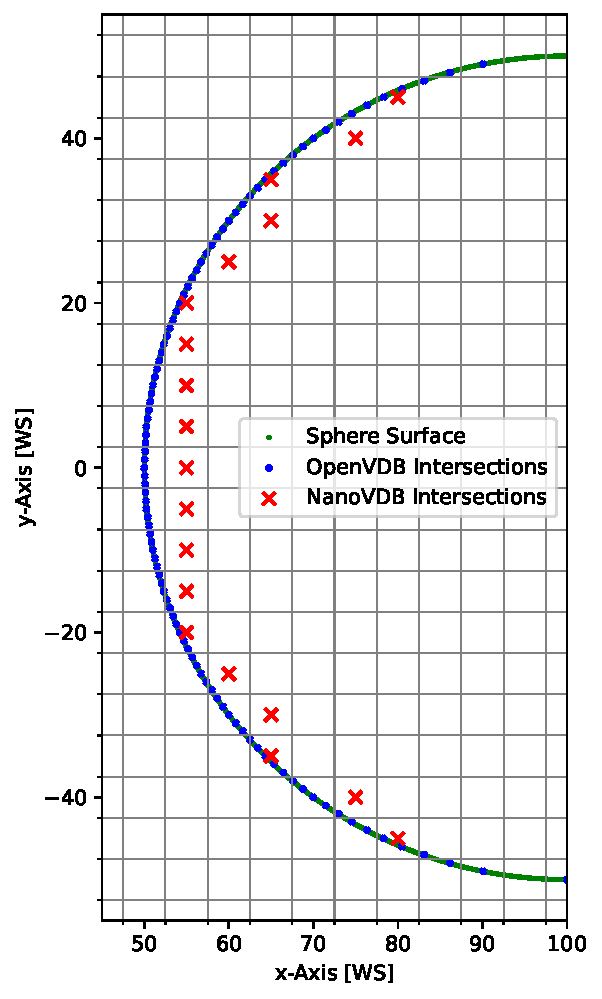
\includegraphics[width=\linewidth]{res/intersection.pdf}
	\endminipage\hfill
	\minipage{0.32\textwidth}
	  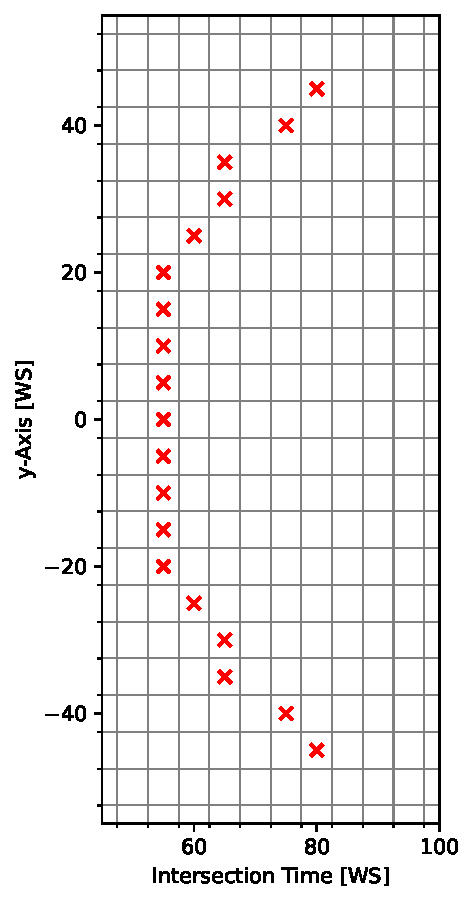
\includegraphics[width=\linewidth]{res/intersection_time.pdf}
	\endminipage\hfill
	\minipage{0.32\textwidth}
	  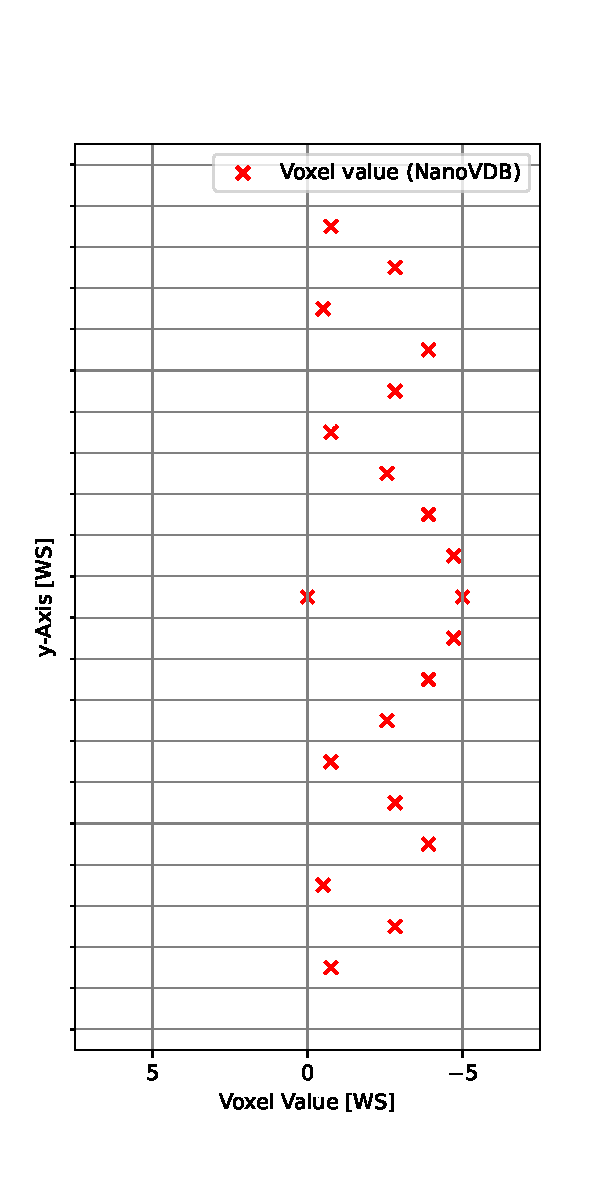
\includegraphics[width=\linewidth]{res/intersection_values.pdf}
	\endminipage
		\caption{ Results of the accuracy experiment. The grid lines resemble voxels. In total 1000 rays are used but many results overlap because the accuracy is reduced to voxel-level
        \textbf{left:} Calculated intersection points compared to analytical solution
		    \textbf{center:} Intersection time/distance
        \textbf{right:} Voxel value at intersection point
        }
	\label{fig:results_accuracy}
\end{figure}





\nocite{openvdb}
\nocite{nanovdb}
